%*****************************************
\chapter{ \textbf{Appendix} }\label{ch:Appendix}
%*****************************************
\vspace{0.5cm} 
%============================================================================================================================================================

\section{SQL-queries}\label{sec:SQL}
\lstset{language = SQL}

In this section, the queries performed in the \textit{Gaia} database are shown for the three different fields of Sco-Cen OB Association namely Lower Centaurus Crux (LCC), Upper Centaurus Lupus (UCL), and Upper Scorpius (US).\\    

\textbf{Lower Centaurus Crux (LCC)}
\begin{lstlisting}[frame = single]
SELECT gaia.source_id, 
gaia.ra, gaia.ra_error, gaia.dec, gaia.dec_error, gaia.parallax, gaia.parallax_error, gaia.l, gaia.b,
gaia.phot_g_mean_mag+5*log10(gaia.parallax)-10 AS g_mag_abs,
tycho2.bt_mag-tycho2.vt_mag AS b_min_v
FROM gaiadr1.tgas_source AS gaia
INNER JOIN tycho2 as tycho2
ON gaia.tycho2_id = tycho2.id
WHERE gaia.parallax >= 6 AND gaia.parallax <= 12 AND gaia.b >= -10 AND gaia.b <= 16 AND gaia.l >= 285 AND gaia.l <= 313

SELECT gaia.source_id, 
gaia.ra, gaia.ra_error, gaia.dec, gaia.dec_error, gaia.parallax, gaia.parallax_error, gaia.l, gaia.b, 
gaia.phot_g_mean_mag+5*log10(gaia.parallax)-10 AS g_mag_abs, 
gaia.phot_g_mean_mag-tmass.ks_m AS g_min_ks, gaia.pmra, gaia.pmra_error, gaia.pmdec, gaia.pmdec_error 
FROM gaiadr1.gaia_source AS gaia INNER JOIN gaiadr1.tmass_best_neighbour AS xmatch ON gaia.source_id = xmatch.source_id 
INNER JOIN gaiadr1.tmass_original_valid AS tmass ON tmass.tmass_oid = xmatch.tmass_oid 
WHERE gaia.parallax >= 6 AND gaia.parallax <= 12 AND gaia.b >= -10 AND gaia.b <= 16 AND gaia.l >= 285 AND gaia.l <= 313 
AND gaia.pmra < 10 AND gaia.pmdec < 30 AND sqrt(power(gaia.pmra,2)+power(gaia.pmdec,2)) > 15 AND sqrt(power(gaia.pmra,2)+power(gaia.pmdec,2)) < 55

SELECT gaia.source_id, 
gaia.ra, gaia.ra_error, gaia.dec, gaia.dec_error, gaia.parallax, gaia.parallax_error, gaia.l, gaia.b, 
gaia.phot_g_mean_mag+5*log10(gaia.parallax)-10 AS g_mag_abs, 
gaia.bp_rp, gaia.pmra, gaia.pmra_error, gaia.pmdec, gaia.pmdec_error, gaia.phot_bp_mean_mag, gaia.phot_rp_mean_mag, gaia.phot_g_mean_mag, 
gaia.astrometric_n_good_obs_al, gaia.astrometric_chi2_al, gaia.phot_bp_mean_flux_over_error, gaia.phot_rp_mean_flux_over_error, 
gaia.phot_bp_rp_excess_factor 
FROM gaiadr2.gaia_source AS gaia 
WHERE gaia.parallax >= 6 AND gaia.parallax <= 12 AND gaia.b >= -10 AND gaia.b <= 16 AND gaia.l >= 285 AND gaia.l <= 313 
AND gaia.pmra < 10 AND gaia.pmdec < 30 AND sqrt(power(gaia.pmra,2)+power(gaia.pmdec,2)) > 15 AND sqrt(power(gaia.pmra,2)+power(gaia.pmdec,2)) < 55 
AND (gaia.parallax/gaia.parallax_error) > 10 AND gaia.phot_bp_mean_flux_over_error > 10 AND gaia.phot_rp_mean_flux_over_error > 10 
AND gaia.phot_bp_rp_excess_factor > (1.0 + 0.015*power((gaia.phot_bp_mean_mag-gaia.phot_rp_mean_mag),2)) 
AND gaia.phot_bp_rp_excess_factor < (1.3 + 0.06*power((gaia.phot_bp_mean_mag-gaia.phot_rp_mean_mag),2))

\end{lstlisting}\vspace{5mm}

\textbf{Upper Centaurus Lupus (UCL)}
\begin{lstlisting}[frame = single]
SELECT gaia.source_id, 
gaia.ra, gaia.ra_error, gaia.dec, gaia.dec_error, gaia.parallax, gaia.parallax_error, gaia.l, gaia.b,
gaia.phot_g_mean_mag+5*log10(gaia.parallax)-10 AS g_mag_abs,
tycho2.bt_mag-tycho2.vt_mag AS b_min_v
FROM gaiadr1.tgas_source AS gaia
INNER JOIN tycho2 as tycho2
ON gaia.tycho2_id = tycho2.id
WHERE gaia.parallax >= 6.0 AND gaia.parallax <= 12 AND gaia.b >= 5 AND gaia.b <= 31 AND gaia.l >= 313 AND gaia.l <= 337

SELECT gaia.source_id, 
gaia.ra, gaia.ra_error, gaia.dec, gaia.dec_error, gaia.parallax, gaia.parallax_error, gaia.l, gaia.b, 
gaia.phot_g_mean_mag+5*log10(gaia.parallax)-10 AS g_mag_abs, 
gaia.phot_g_mean_mag-tmass.ks_m AS g_min_ks, gaia.pmra, gaia.pmra_error, gaia.pmdec, gaia.pmdec_error 
FROM gaiadr1.gaia_source AS gaia INNER JOIN gaiadr1.tmass_best_neighbour AS xmatch ON gaia.source_id = xmatch.source_id 
INNER JOIN gaiadr1.tmass_original_valid AS tmass ON tmass.tmass_oid = xmatch.tmass_oid 
WHERE gaia.parallax >= 6.0 AND gaia.parallax <= 12 AND gaia.b >= 5 AND gaia.b <= 31 AND gaia.l >= 313 AND gaia.l <= 337 
AND gaia.pmra < 10 AND gaia.pmdec < 30 AND sqrt(power(gaia.pmra,2)+power(gaia.pmdec,2)) > 12 AND sqrt(power(gaia.pmra,2)+power(gaia.pmdec,2)) < 55

SELECT gaia.source_id, 
gaia.ra, gaia.ra_error, gaia.dec, gaia.dec_error, gaia.parallax, gaia.parallax_error, gaia.l, gaia.b, 
gaia.phot_g_mean_mag+5*log10(gaia.parallax)-10 AS g_mag_abs,
gaia.bp_rp, gaia.pmra, gaia.pmra_error, gaia.pmdec, gaia.pmdec_error, gaia.phot_bp_mean_mag, gaia.phot_rp_mean_mag, gaia.phot_g_mean_mag, 
gaia.astrometric_n_good_obs_al, gaia.astrometric_chi2_al, gaia.phot_bp_mean_flux_over_error, gaia.phot_rp_mean_flux_over_error, 
gaia.phot_bp_rp_excess_factor 
FROM gaiadr2.gaia_source AS gaia 
WHERE gaia.parallax >= 6.0 AND gaia.parallax <= 12 AND gaia.b >= 5 AND gaia.b <= 31 AND gaia.l >= 313 AND gaia.l <= 337 
AND gaia.pmra < 10 AND gaia.pmdec < 30 AND sqrt(power(gaia.pmra,2)+power(gaia.pmdec,2)) > 12 AND sqrt(power(gaia.pmra,2)+power(gaia.pmdec,2)) < 55 
AND (gaia.parallax/gaia.parallax_error) > 10 AND gaia.phot_bp_mean_flux_over_error > 10 AND gaia.phot_rp_mean_flux_over_error > 10 
AND gaia.phot_bp_rp_excess_factor > (1.0 + 0.015*power((gaia.phot_bp_mean_mag-gaia.phot_rp_mean_mag),2)) 
AND gaia.phot_bp_rp_excess_factor < (1.3 + 0.06*power((gaia.phot_bp_mean_mag-gaia.phot_rp_mean_mag),2))

\end{lstlisting}\vspace{5mm}

\textbf{Upper Scorpius (US)}
\begin{lstlisting}[frame = single]
SELECT gaia.source_id, 
gaia.ra, gaia.ra_error, gaia.dec, gaia.dec_error, gaia.parallax, gaia.parallax_error, gaia.l, gaia.b,
gaia.phot_g_mean_mag+5*log10(gaia.parallax)-10 AS g_mag_abs,
tycho2.bt_mag-tycho2.vt_mag AS b_min_v
FROM gaiadr1.tgas_source AS gaia
INNER JOIN tycho2 as tycho2
ON gaia.tycho2_id = tycho2.id
WHERE gaia.parallax >= 6.0 AND gaia.parallax <= 12 AND gaia.b >= 7 AND gaia.b <= 32 AND gaia.l >= 337 AND gaia.l <= 360

SELECT gaia.source_id, 
gaia.ra, gaia.ra_error, gaia.dec, gaia.dec_error, gaia.parallax, gaia.parallax_error, gaia.l, gaia.b,
gaia.phot_g_mean_mag+5*log10(gaia.parallax)-10 AS g_mag_abs, 
gaia.phot_g_mean_mag-tmass.ks_m AS g_min_ks, gaia.pmra, gaia.pmra_error, gaia.pmdec, gaia.pmdec_error 
FROM gaiadr1.gaia_source AS gaia INNER JOIN gaiadr1.tmass_best_neighbour AS xmatch ON gaia.source_id = xmatch.source_id 
INNER JOIN gaiadr1.tmass_original_valid AS tmass ON tmass.tmass_oid = xmatch.tmass_oid 
WHERE gaia.parallax >= 6.0 AND gaia.parallax <= 12 AND gaia.b >= 7 AND gaia.b <= 32 AND gaia.l >= 337 AND gaia.l <= 360 
AND gaia.pmra < 10 AND gaia.pmdec < 30 AND sqrt(power(gaia.pmra,2)+power(gaia.pmdec,2)) < 47

SELECT gaia.source_id, 
gaia.ra, gaia.ra_error, gaia.dec, gaia.dec_error, gaia.parallax, gaia.parallax_error, gaia.l, gaia.b, 
gaia.phot_g_mean_mag+5*log10(gaia.parallax)-10 AS g_mag_abs, 
gaia.bp_rp, gaia.pmra, gaia.pmra_error, gaia.pmdec, gaia.pmdec_error, gaia.phot_bp_mean_mag, gaia.phot_rp_mean_mag, gaia.phot_g_mean_mag, 
gaia.astrometric_n_good_obs_al, gaia.astrometric_chi2_al, gaia.phot_bp_mean_flux_over_error, 
gaia.phot_rp_mean_flux_over_error, gaia.phot_bp_rp_excess_factor 
FROM gaiadr2.gaia_source AS gaia 
WHERE gaia.parallax >= 6.0 AND gaia.parallax <= 12 AND gaia.b >= 7 AND gaia.b <= 32 AND gaia.l >= 337 AND gaia.l <= 360 
AND gaia.pmra < 10 AND gaia.pmdec < 30 AND sqrt(power(gaia.pmra,2)+power(gaia.pmdec,2)) < 47 AND (gaia.parallax/gaia.parallax_error) > 10 
AND gaia.phot_bp_mean_flux_over_error > 10 AND gaia.phot_rp_mean_flux_over_error > 10 
AND gaia.phot_bp_rp_excess_factor > (1.0 + 0.015*power((gaia.phot_bp_mean_mag-gaia.phot_rp_mean_mag),2)) 
AND gaia.phot_bp_rp_excess_factor < (1.3 + 0.06*power((gaia.phot_bp_mean_mag-gaia.phot_rp_mean_mag),2))
\end{lstlisting}\vspace{5mm}

\textbf{ScoCen Pre-Main Sequence Population}
\begin{lstlisting}[frame = single]
SELECT gaia.source_id, gaia.ra, gaia.ra_error, gaia.dec, gaia.dec_error, gaia.parallax, gaia.parallax_error, gaia.l, gaia.b, 
gaia.phot_g_mean_mag+5*log10(gaia.parallax)-10.0 AS g_mag_abs, 
gaia.bp_rp, gaia.pmra, gaia.pmra_error, gaia.pmdec, gaia.pmdec_error, gaia.phot_bp_mean_mag, gaia.phot_rp_mean_mag, gaia.phot_g_mean_mag, 
gaia.astrometric_n_good_obs_al, gaia.astrometric_chi2_al, gaia.phot_bp_mean_flux_over_error, 
gaia.phot_rp_mean_flux_over_error, gaia.phot_bp_rp_excess_factor,
gaia.visibility_periods_used, (gaia.astrometric_chi2_al/(gaia.astrometric_n_good_obs_al - 5.0)) AS unit_weight 
FROM gaiadr2.gaia_source AS gaia 
WHERE gaia.parallax >= 5.0 AND gaia.parallax <= 12.0 AND gaia.b >= -10.0 AND gaia.b <= 32.0 AND gaia.l >= 285.0 AND gaia.l <= 360.0 
AND (gaia.parallax/gaia.parallax_error) > 10.0 AND gaia.phot_bp_mean_flux_over_error > 10 AND gaia.phot_rp_mean_flux_over_error > 10 
AND gaia.phot_bp_rp_excess_factor > (1.0 + 0.015*power((gaia.phot_bp_mean_mag-gaia.phot_rp_mean_mag),2)) 
AND gaia.phot_bp_rp_excess_factor < (1.3 + 0.06*power((gaia.phot_bp_mean_mag-gaia.phot_rp_mean_mag),2))
\end{lstlisting}

\section{Sample selection}\label{sec:Sample_Selection_1}

\begin{figure}[!ht]
\centering
  \subfloat{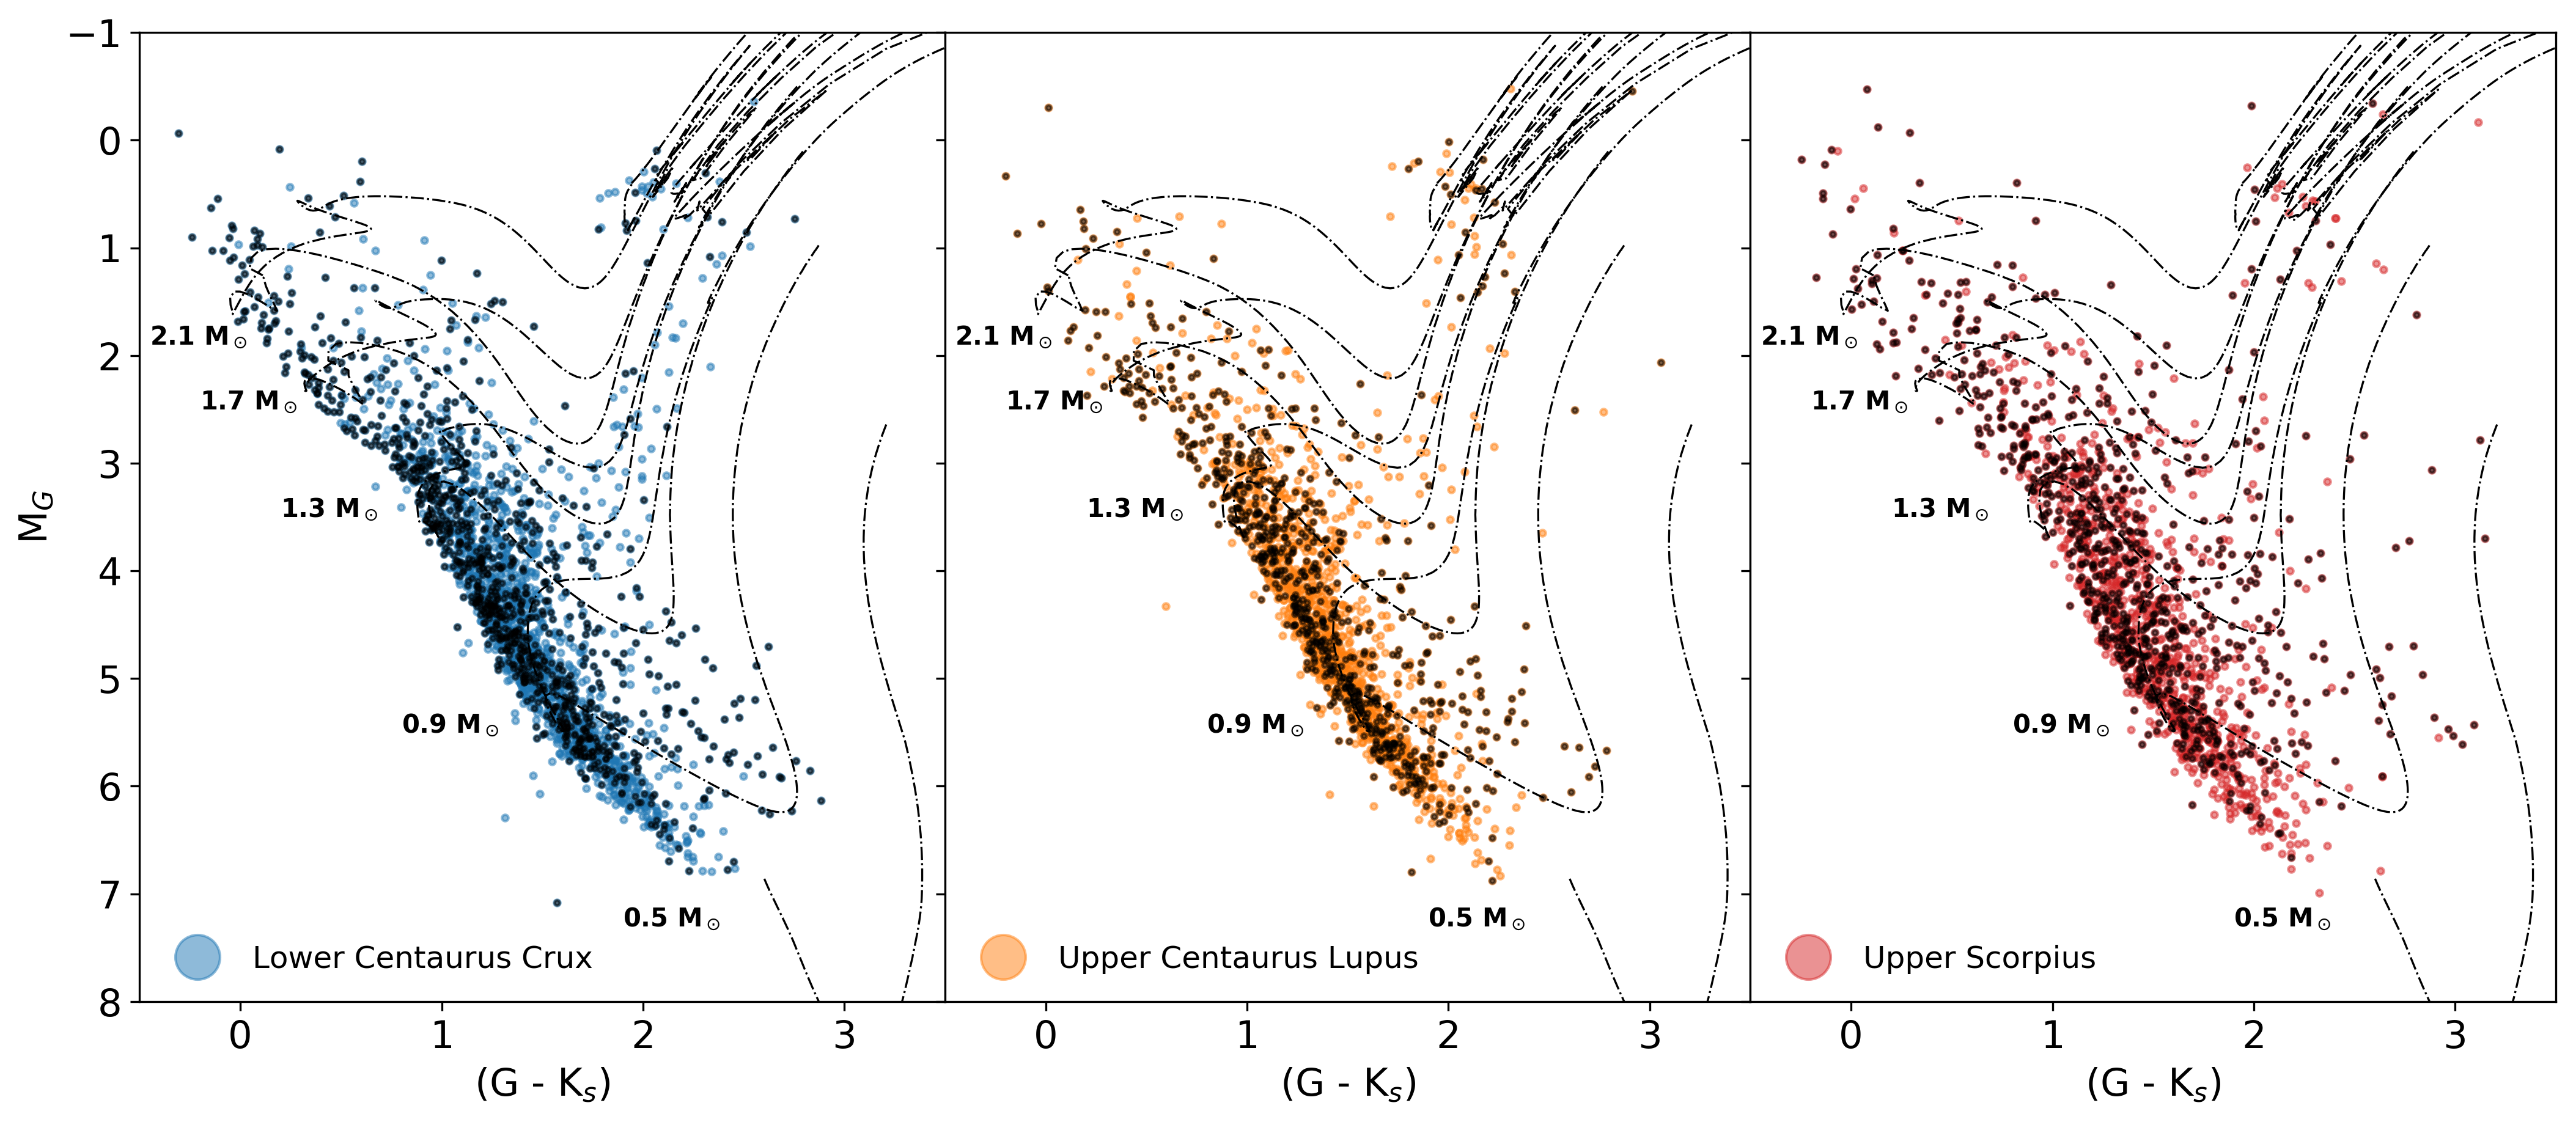
\includegraphics[width = 15cm, height = 6.5cm]{./Graficos/Capitulo_3/5_Sco-Cen/Mag_Col_diagram_4.png}} 
\caption{\scriptsize{Color-magnitude diagrams for each subgroup in ScoCen using \textit{Gaia}-DR1 data. \textit{\textbf{Left}}: LCC stars after the dynamical and positional cuts are shown in blue. The black lines correspond to different stellar tracks. \textit{\textbf{\textbf{Center}}}: UCL stars after the dynamical and positional cuts are shown in orange. The black lines correspond to different stellar tracks. \textit{\textbf{Right}}: US stars after the dynamical and positional cuts are shown in red. The black lines correspond to different stellar tracks. In general for each subgroup, a stellar mass range of $0.5 \textnormal{M}_\odot < \textnormal{M} < 2.1 \textnormal{M}_\odot$ was used along with $\textnormal{A}_\textnormal{v} = 0$ using the \textit{MIST}-package (\cauthor{2016ApJS..222....8D} \citeyear{2016ApJS..222....8D}; \cauthor{2016ApJ...823..102C} \citeyear{2016ApJ...823..102C}).}}
\label{fig:Stellar_Tracks_1_appendix}
\end{figure}

\begin{figure}[!ht]
\centering
  \subfloat{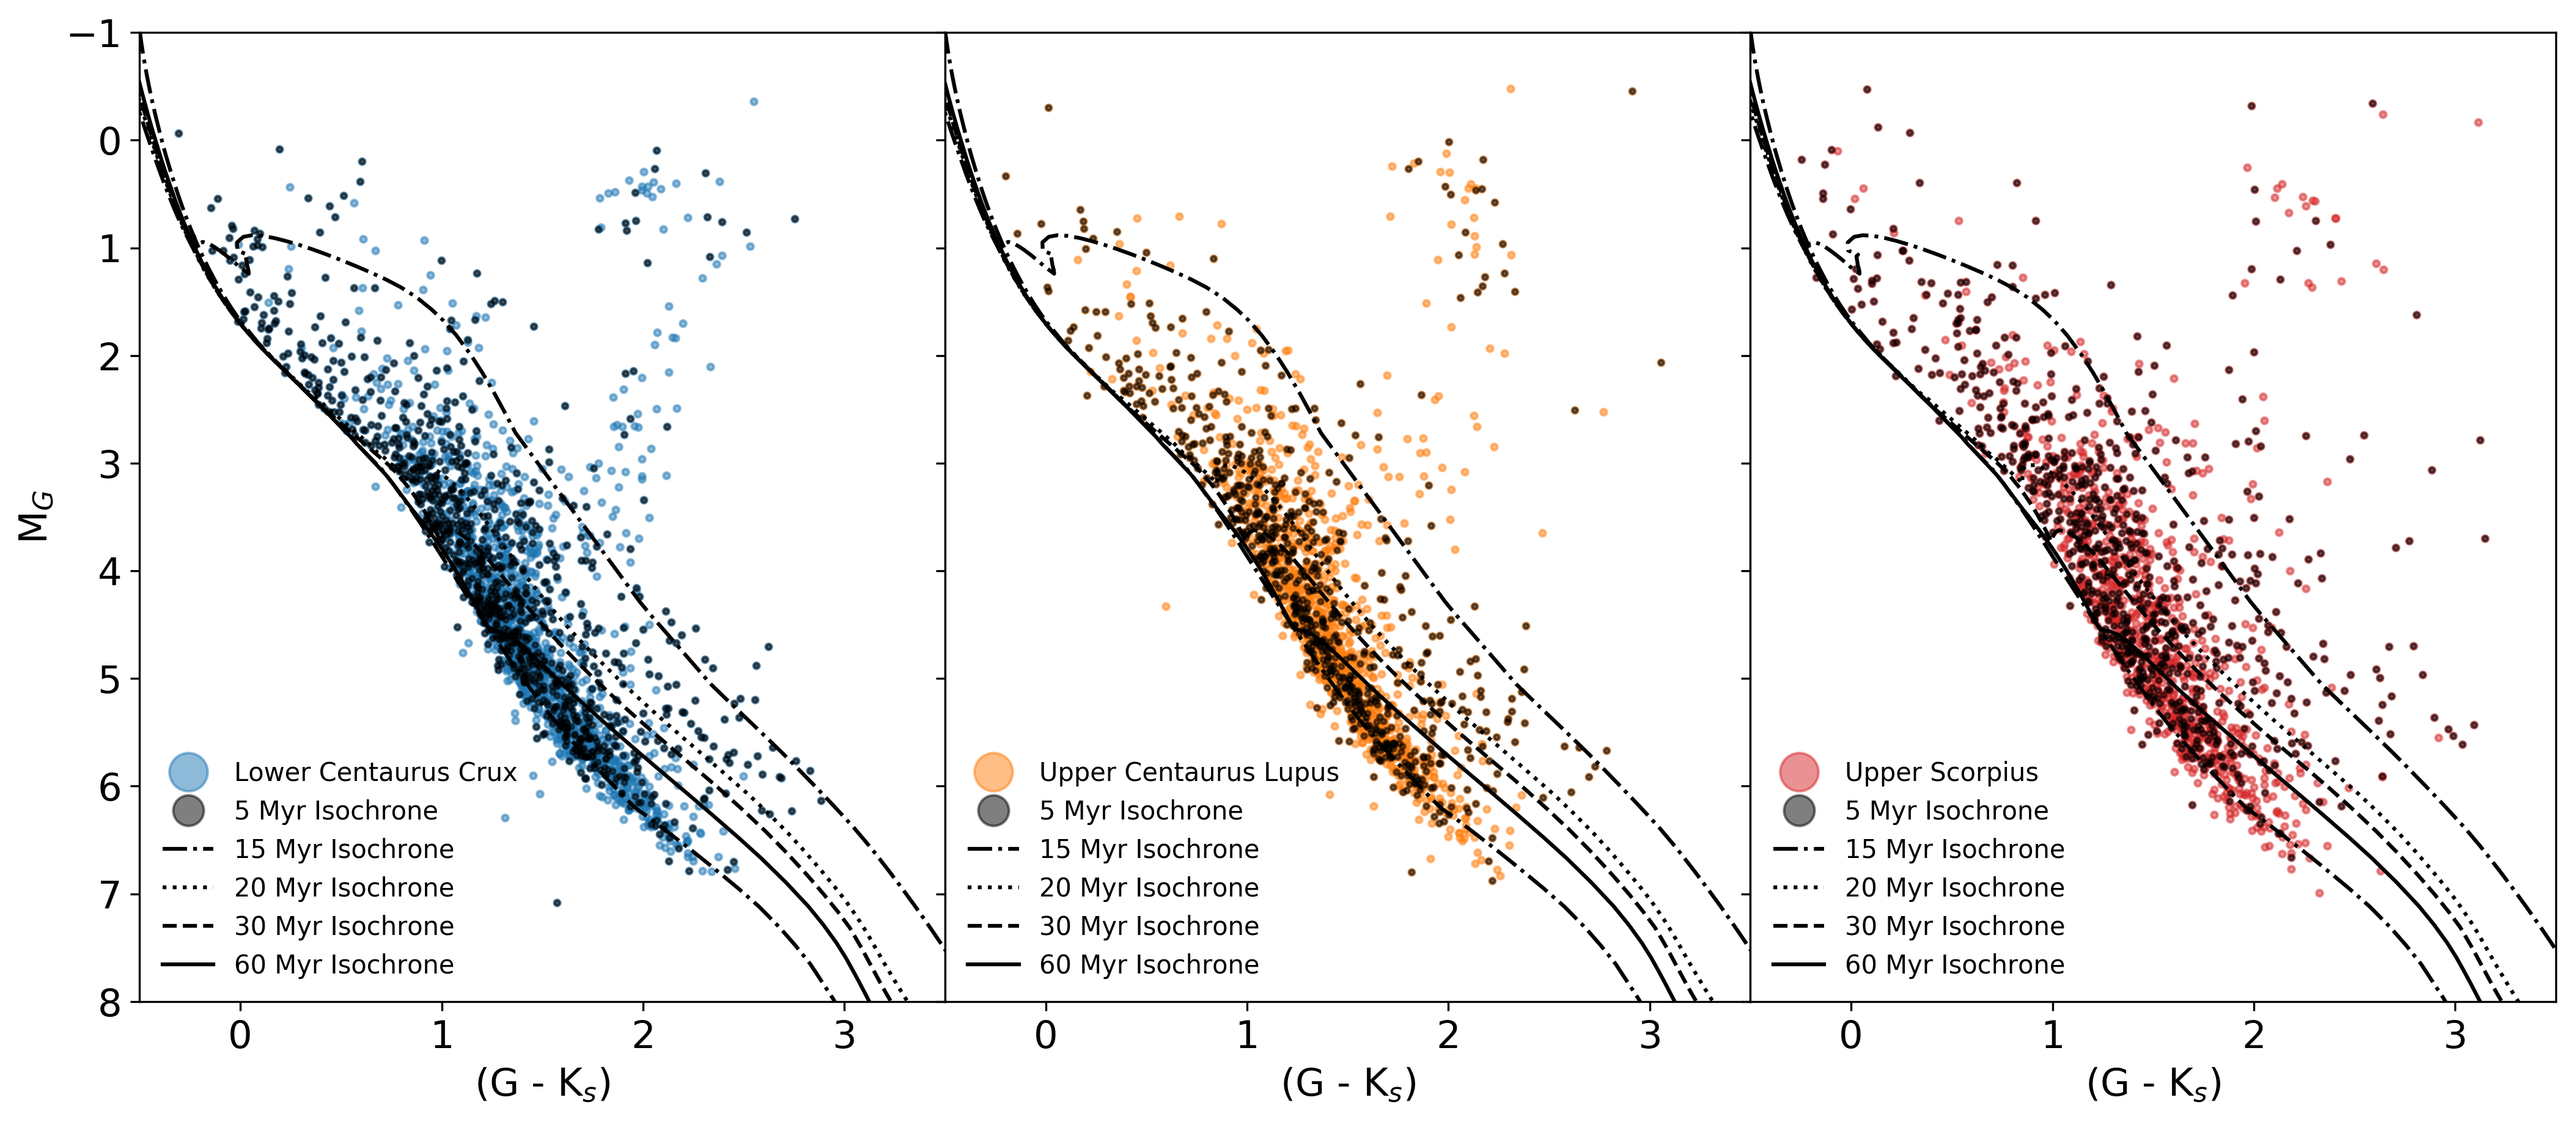
\includegraphics[width = 15cm, height = 6.5cm]{./Graficos/Capitulo_3/5_Sco-Cen/Mag_Col_diagram_3.png}} 
\caption{\scriptsize{Color-magnitude diagrams for each subgroup in ScoCen using \textit{Gaia}-DR1 data. \textit{\textbf{Left}}: LCC stars after the dynamical and positional cuts are shown in blue. The black lines correspond to different isochrones. \textit{\textbf{Center}}: UCL stars after the dynamical and positional cuts are shown in orange. The black lines correspond to different isochrones. \textit{\textbf{Right}}: US stars after the dynamical and positional cuts are shown in red. The black lines correspond to different isochrones. In general for each subgroup, isochrones from $5 \textnormal{Myr}$ to $60 \textnormal{Myr}$ were calculated along with $\textnormal{A}_\textnormal{v} = 0$ using the \textit{MIST}-package (\cauthor{2016ApJS..222....8D} \citeyear{2016ApJS..222....8D}; \cauthor{2016ApJ...823..102C} \citeyear{2016ApJ...823..102C}). The $60 \textnormal{Myr}$ isochrone fits well the main-sequence and the $5 \textnormal{Myr}$ isochrones gives a good range to pre-select young stars. The black dots are the final sample after the isochrone selection.}}
\label{fig:Isochrones_1_appendix}
\end{figure}

\begin{figure}[!ht]
\centering
  \subfloat{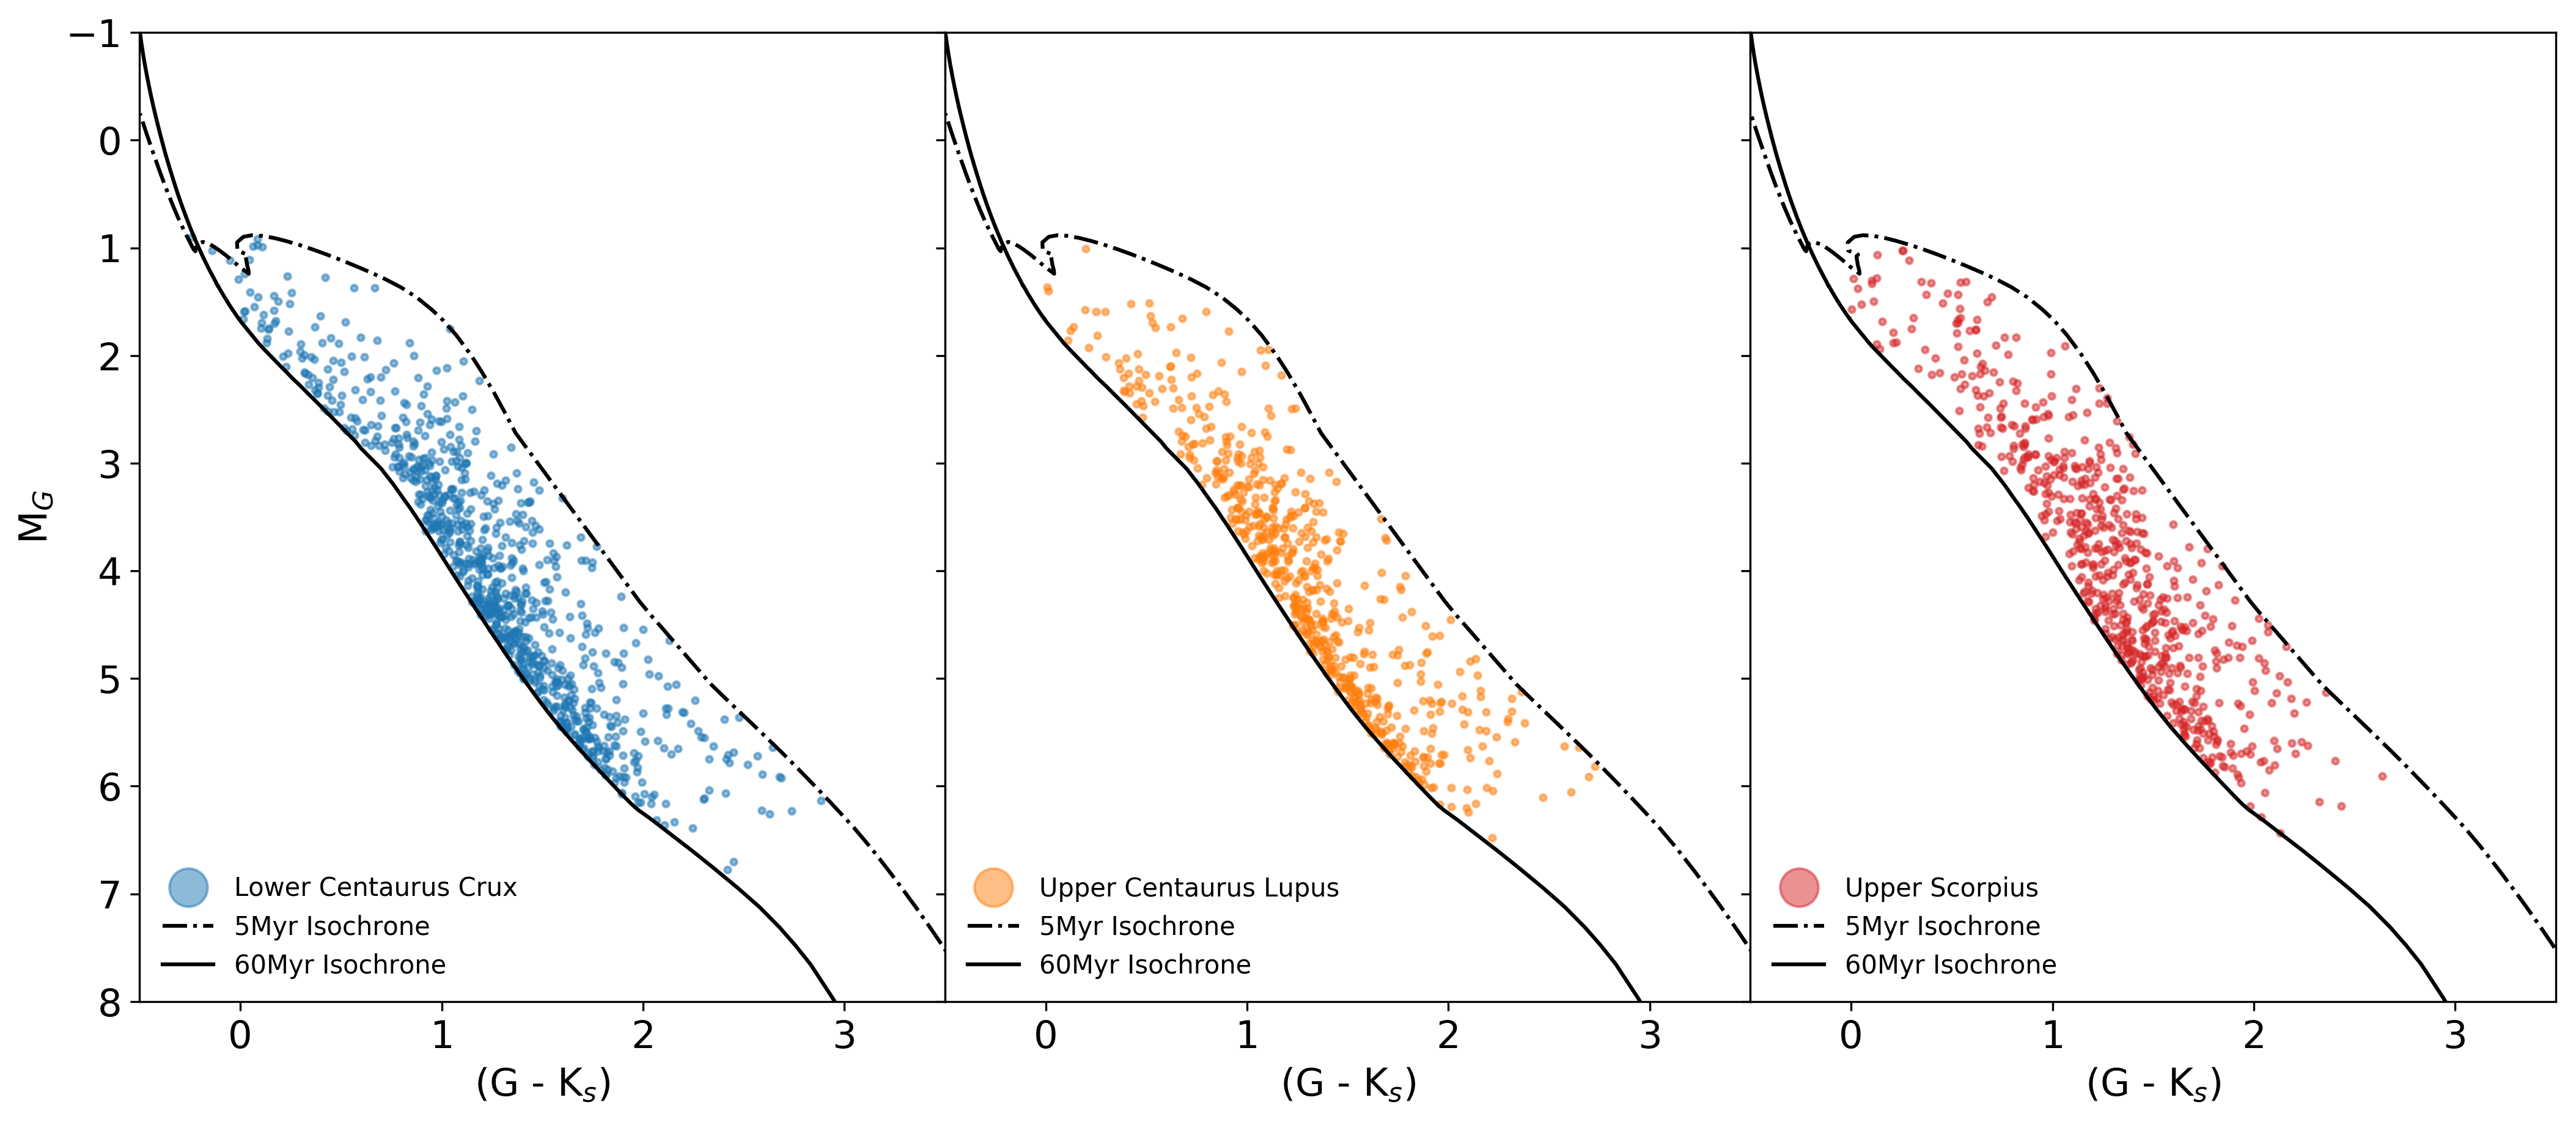
\includegraphics[width = 15cm, height = 6.5cm]{./Graficos/Capitulo_3/5_Sco-Cen/final_Sample_SCOCEN_Original.png}} 
\caption{\scriptsize{Color-magnitude diagrams for each subgroup in ScoCen using selected \textit{Gaia}-DR1 data between two different isochrones. \textit{\textbf{Left}}: LCC stars after the dynamical and positional cuts are shown in blue. The black lines correspond to different isochrones. \textit{\textbf{Center}}: UCL stars after the dynamical and positional cuts are shown in orange. The black lines correspond to different isochrones. \textit{\textbf{Right}}: US stars after the dynamical and positional cuts are shown in red. The black lines correspond to different isochrones. Only the $5 \textnormal{Myr}$ to $60 \textnormal{Myr}$ isochrones were used with $\textnormal{A}_\textnormal{v} = 0$ to restrict the sample of stars to be inside this particular region. Following this, stars inside the region are quite likely to belong to the cluster and be in an stellar age range suitable for our study. The black dots are the final sample after the isochrone selection.}}
\label{fig:Isochrones_2}
\end{figure}

\begin{figure}[!ht]
\centering
  \subfloat{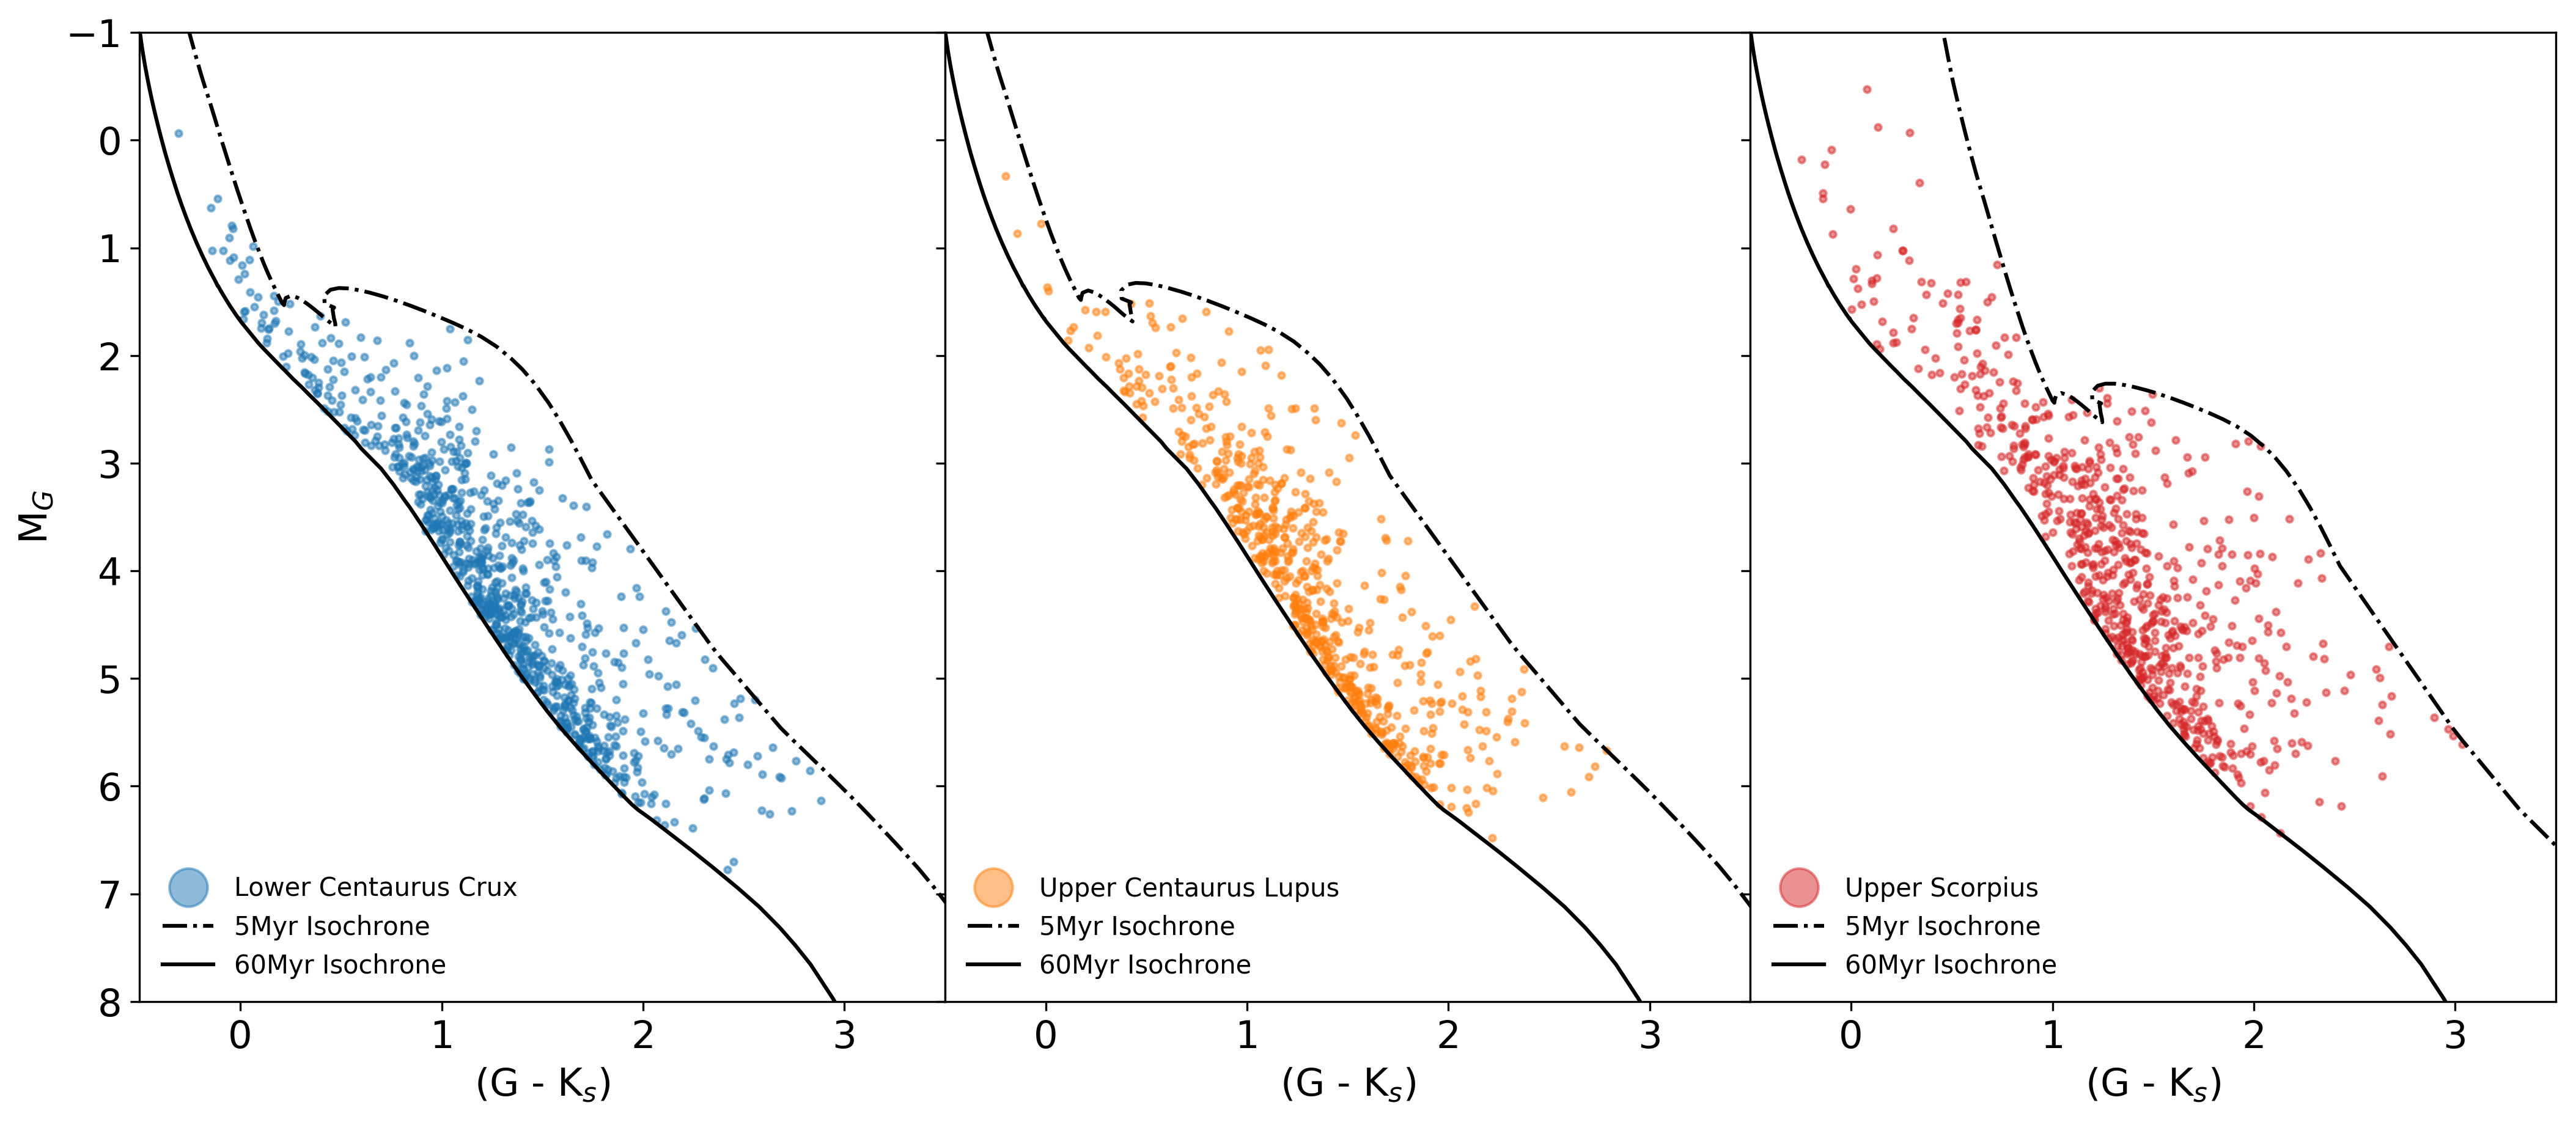
\includegraphics[width = 15cm, height = 6.5cm]{./Graficos/Capitulo_3/5_Sco-Cen/final_Sample_SCOCEN.png}} 
\caption{\scriptsize{Color-magnitude diagrams for each subgroup in ScoCen using selected \textit{Gaia}-DR1 data between two different isochrones as in \autoref{fig:Isochrones_2}, along with isochrones using the extinction value measured proposed by \cauthor{1989A&A...216...44D} (\citeyear{1989A&A...216...44D}). \textit{\textbf{Left}}: LCC stars after the dynamical and positional cuts are shown in blue. The black lines correspond to different isochrones. \textit{\textbf{Center}}: UCL stars after the dynamical and positional cuts are shown in orange. The black lines correspond to different isochrones. \textit{\textbf{Right}}: US stars after the dynamical and positional cuts are shown in red. The black lines correspond to different isochrones. Only the $5 \textnormal{Myr}$ to $60 \textnormal{Myr}$ isochrones were used to restrict the sample of stars to be inside this particular region. Following this, stars inside the region are quite likely to belong to the cluster and be in an stellar age range suitable for our study. In this case, the extinction values for LCC, UCL, and US correspond to $\textnormal{A}_\textnormal{v} = 0.23$, $\textnormal{A}_\textnormal{v} = 0.17$, and $\textnormal{A}_\textnormal{v} = 0.76$, respectively.}}
\label{fig:Isochrones_4}
\end{figure}

\begin{figure}[!ht]
\centering
  \subfloat{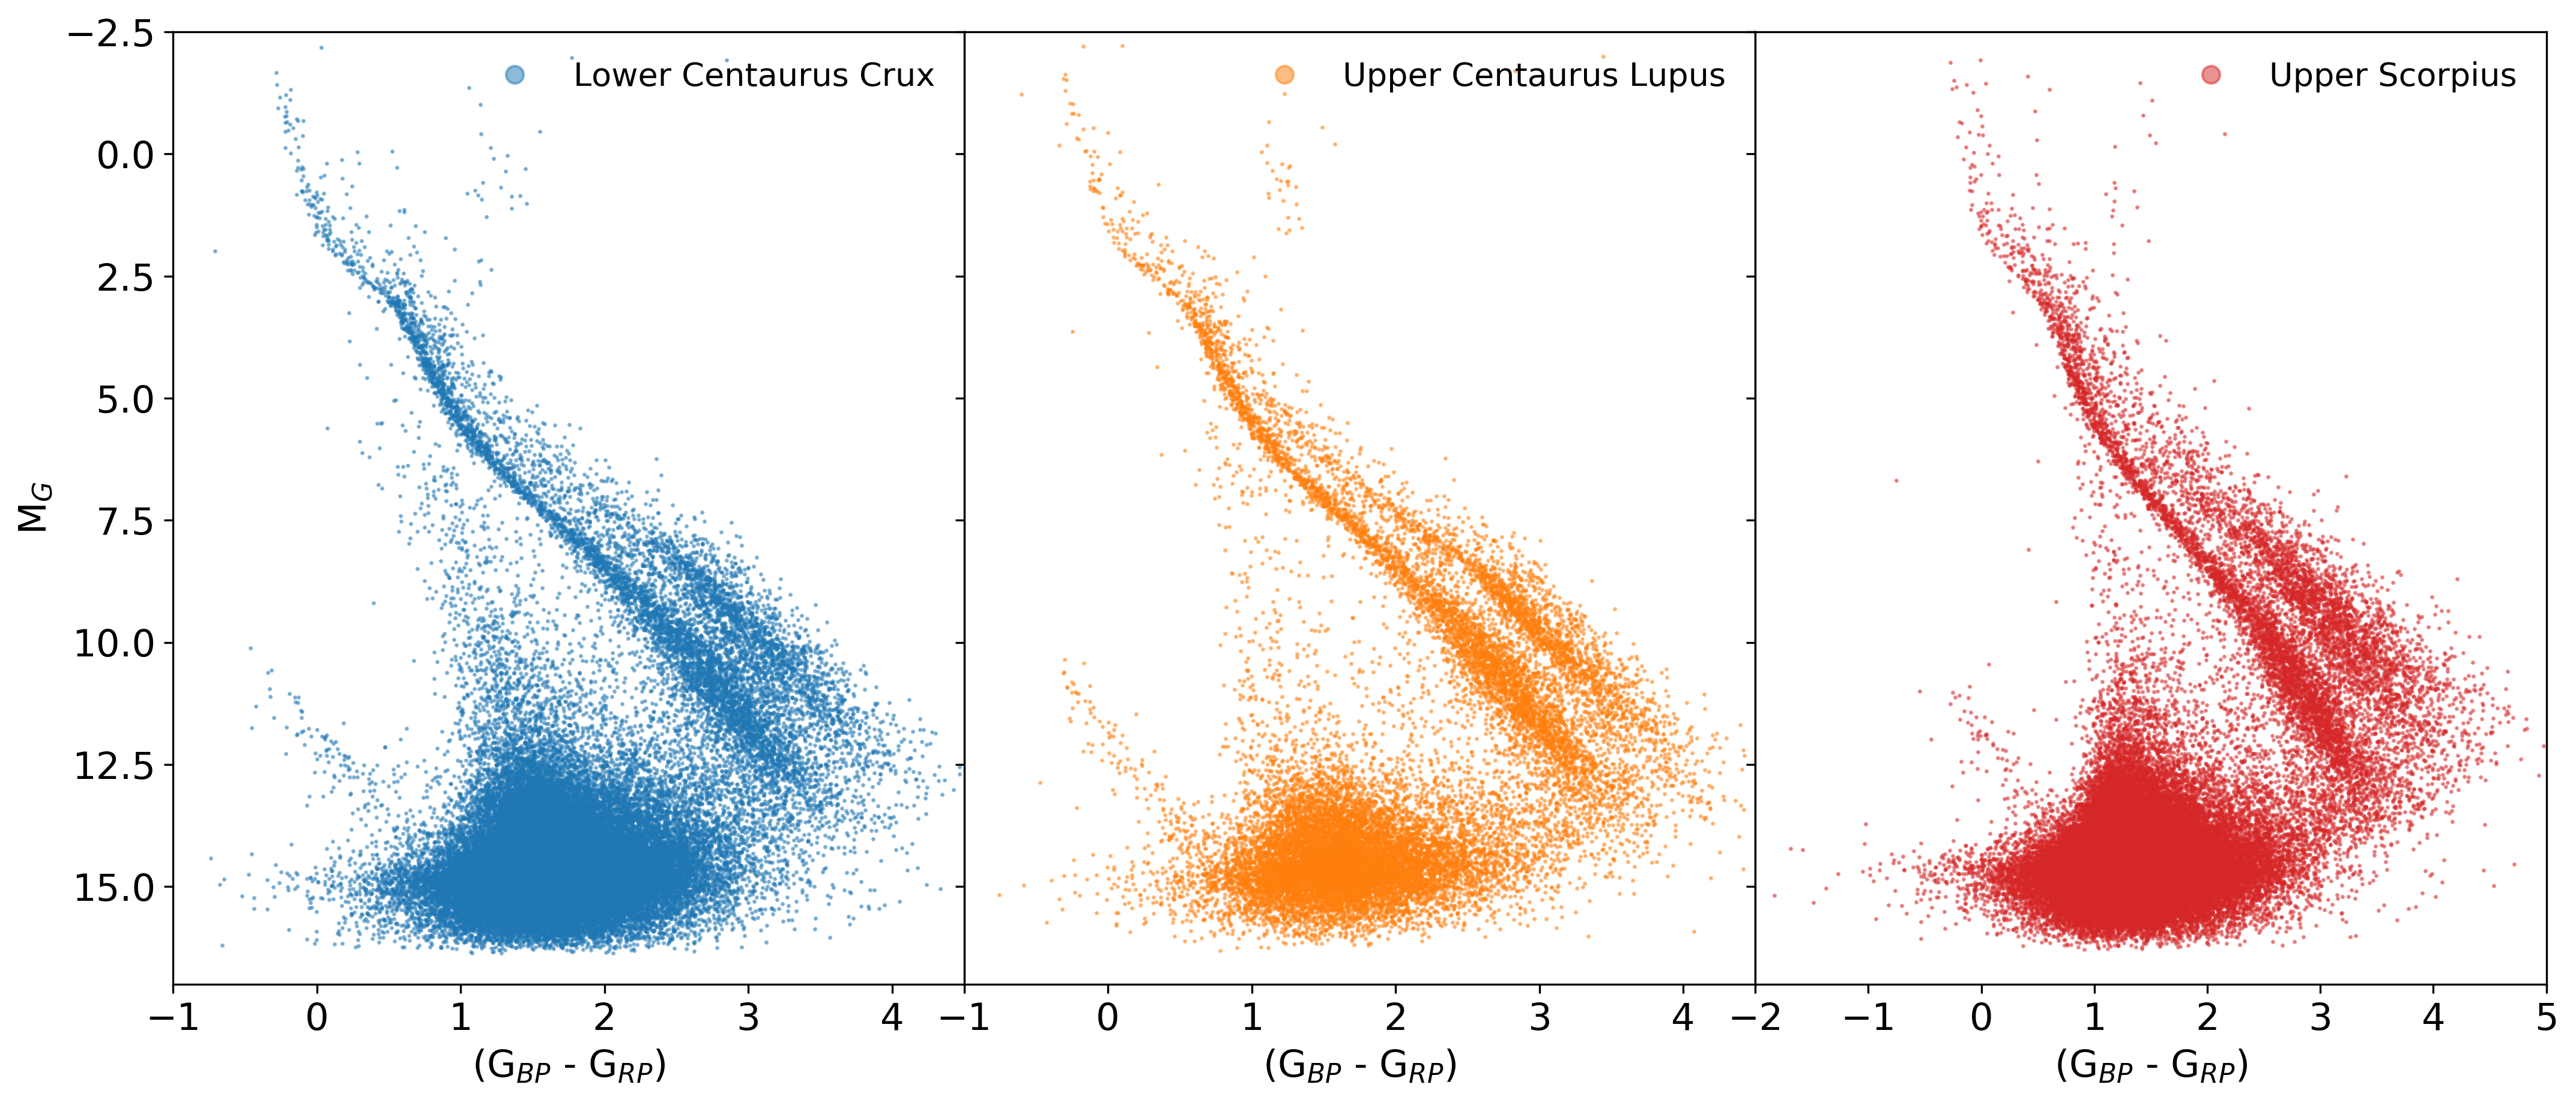
\includegraphics[width = 15cm, height = 6.5cm]{./Graficos/Capitulo_3/7_DR2_LightCurves/DR2_Sample_NoSelection_2_2.png}} 
\caption{\scriptsize{Color-magnitude diagram using \textit{Gaia}-DR2 data for each subgroup in ScoCen. \textit{\textbf{Left}}: LCC absolute magnitude in the $\textnormal{G}$-band as a function of color-index $\textnormal{G}_\textnormal{BP} - \textnormal{G}_\textnormal{RP}$. \textit{\textbf{Center}}: UCL absolute magnitude in the $\textnormal{G}$-band as a function of color-index $\textnormal{G}_\textnormal{BP} - \textnormal{G}_\textnormal{RP}$. \textit{\textbf{Right}}: US absolute magnitude in the $\textnormal{G}$-band as a function of color-index $\textnormal{G}_\textnormal{BP} - \textnormal{G}_\textnormal{RP}$. In contrast to \textit{Gaia}-DR1, the new data sample contains more stars in each subgroup, and stars with absolute magnitude up to $\textnormal{M}_\textnormal{G} > 17$.}}
\label{fig:NewData_DR2}
\end{figure}

\begin{figure}[!ht]
\centering
  \subfloat{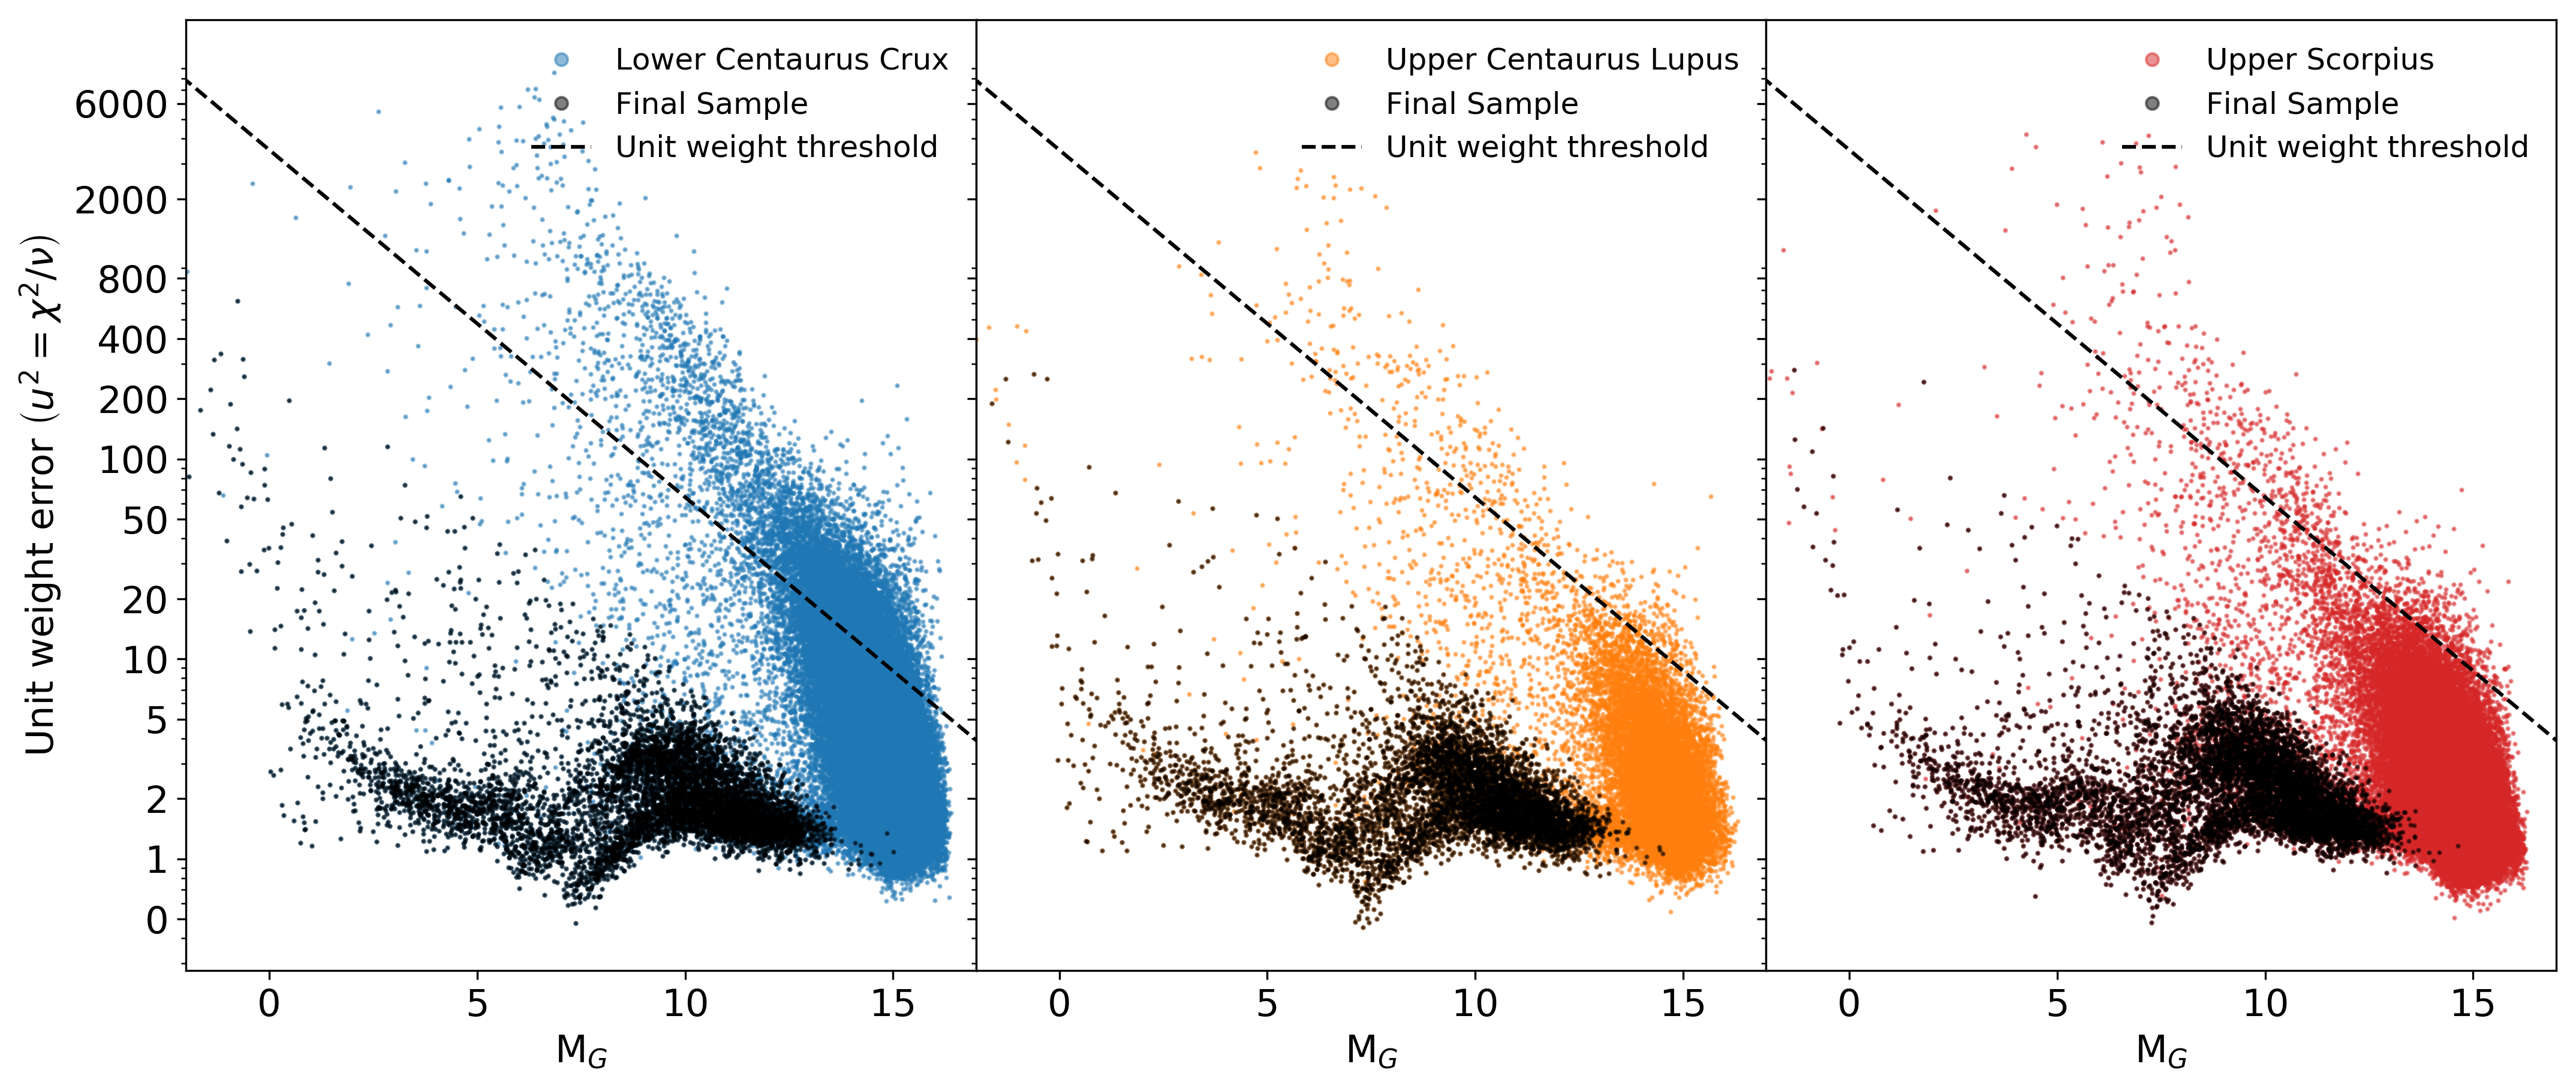
\includegraphics[width = 15cm, height = 6.5cm]{./Graficos/Capitulo_3/7_DR2_LightCurves/Lindegren_Selection.png}} 
\caption{\scriptsize{Unit weight error threshold as proposed by \cauthor{2016ApJS..222....8D} (\citeyear{2016ApJS..222....8D}) to obtain photometric and astrometric cleaned data. The black line represents the threshold defined in \autoref{eq:WeightError}. \textit{\textbf{Left}}: LCC unit weight error as a function of magnitude in the $\textnormal{G}$-band. The blue dots represents the original sample as shown in \autoref{fig:NewData_DR2}-left panel, while the black dots correspond to the filtered by unit weight error and flux excess ratio. \textit{\textbf{Center}}: UCL unit weight error as a function of magnitude in the $\textnormal{G}$-band. The orange dots represents the original sample as shown in \autoref{fig:NewData_DR2}-center panel, while the black dots correspond to the filtered by unit weight error and flux excess ratio. \textit{\textbf{Right}}: US unit weight error as a function of magnitude in the $\textnormal{G}$-band. The red dots represents the original sample as shown in \autoref{fig:NewData_DR2}-right panel, while the black dots correspond to the filtered by unit weight error and flux excess ratio.}}
\label{fig:LindegrenSelection}
\end{figure}

\begin{figure}[!ht]
\centering
  \subfloat{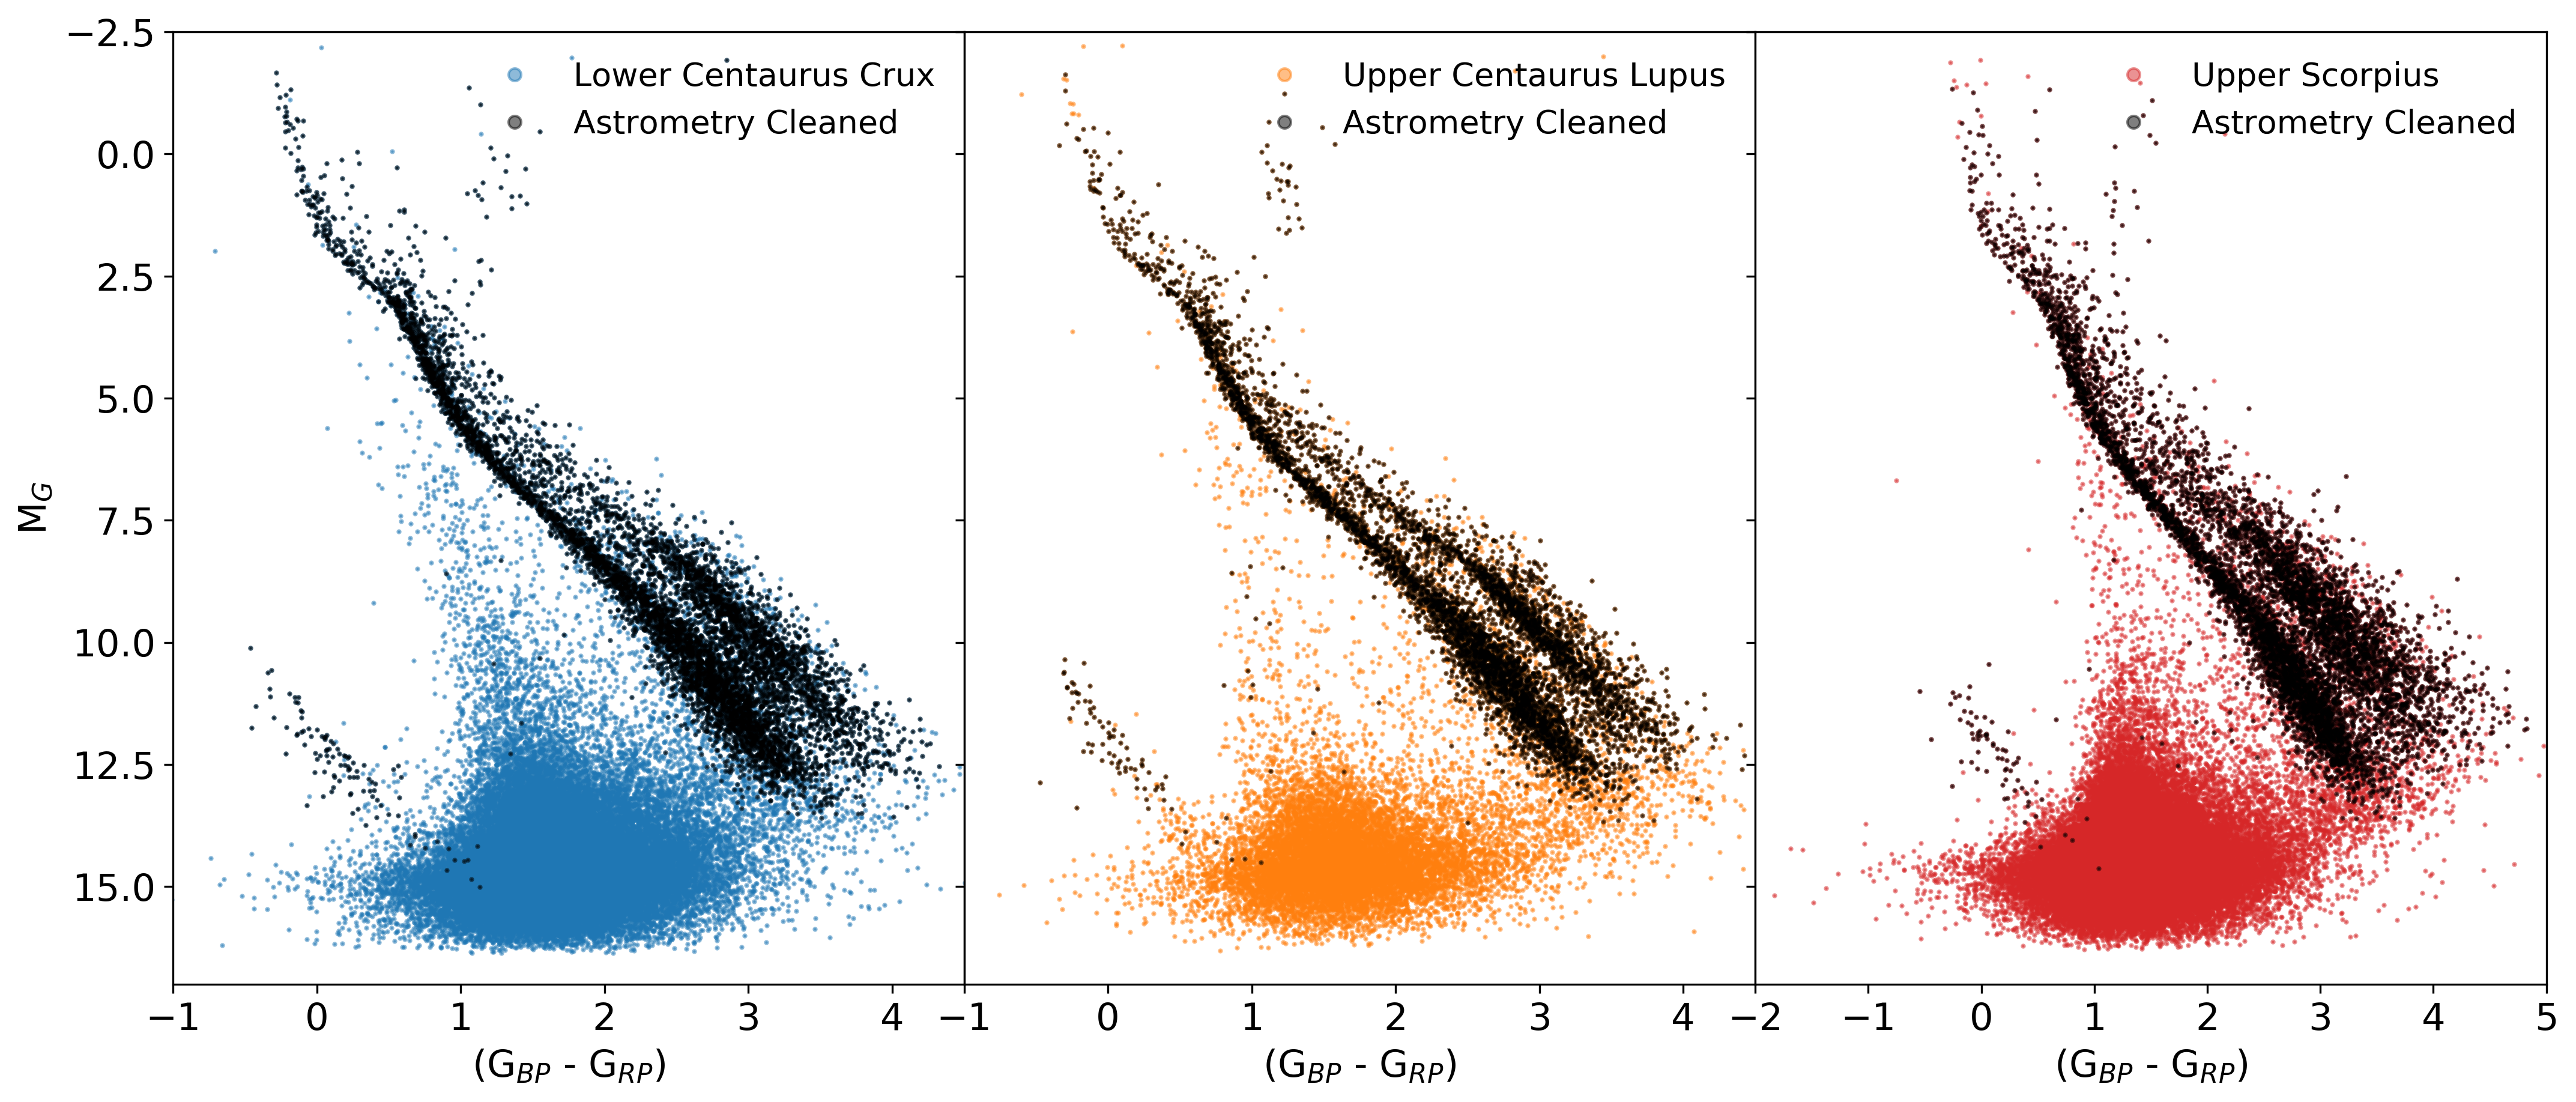
\includegraphics[width = 15cm, height = 6.5cm]{./Graficos/Capitulo_3/7_DR2_LightCurves/CMD_Cleaned_MG.png}} 
\caption{\scriptsize{Color-magnitude diagram using \textit{Gaia}-DR2 data for each subgroup in ScoCen filtered by unit weight error and flux excess ratio. \textit{Left}: LCC absolute magnitude in the $\textnormal{G}$-band as a function of color-index $\textnormal{G}_\textnormal{BP} - \textnormal{G}_\textnormal{RP}$. \textit{\textbf{Center}}: UCL absolute magnitude in the $\textnormal{G}$-band as a function of color-index $\textnormal{G}_\textnormal{BP} - \textnormal{G}_\textnormal{RP}$. \textit{\textbf{Right}}: US absolute magnitude in the $\textnormal{G}$-band as a function of color-index $\textnormal{G}_\textnormal{BP} - \textnormal{G}_\textnormal{RP}$. The color dots show the original sample as presented in \autoref{fig:NewData_DR2}, while the black dots correspond to the final sample after correcting the flux excess ratio and unit weight error as shown in \autoref{fig:LindegrenSelection}.}}
\label{fig:FinalSample_DR2}
\end{figure}
